\documentclass[man]{apa6}
\usepackage{lmodern}
\usepackage{amssymb,amsmath}
\usepackage{ifxetex,ifluatex}
\usepackage{fixltx2e} % provides \textsubscript
\ifnum 0\ifxetex 1\fi\ifluatex 1\fi=0 % if pdftex
  \usepackage[T1]{fontenc}
  \usepackage[utf8]{inputenc}
\else % if luatex or xelatex
  \ifxetex
    \usepackage{mathspec}
  \else
    \usepackage{fontspec}
  \fi
  \defaultfontfeatures{Ligatures=TeX,Scale=MatchLowercase}
\fi
% use upquote if available, for straight quotes in verbatim environments
\IfFileExists{upquote.sty}{\usepackage{upquote}}{}
% use microtype if available
\IfFileExists{microtype.sty}{%
\usepackage{microtype}
\UseMicrotypeSet[protrusion]{basicmath} % disable protrusion for tt fonts
}{}
\usepackage{hyperref}
\hypersetup{unicode=true,
            pdftitle={Results Draft},
            pdfauthor={Karen Santamaria, Yifan Ma, Caroline Li, \& Jane Bang},
            pdfborder={0 0 0},
            breaklinks=true}
\urlstyle{same}  % don't use monospace font for urls
\usepackage{graphicx,grffile}
\makeatletter
\def\maxwidth{\ifdim\Gin@nat@width>\linewidth\linewidth\else\Gin@nat@width\fi}
\def\maxheight{\ifdim\Gin@nat@height>\textheight\textheight\else\Gin@nat@height\fi}
\makeatother
% Scale images if necessary, so that they will not overflow the page
% margins by default, and it is still possible to overwrite the defaults
% using explicit options in \includegraphics[width, height, ...]{}
\setkeys{Gin}{width=\maxwidth,height=\maxheight,keepaspectratio}
\IfFileExists{parskip.sty}{%
\usepackage{parskip}
}{% else
\setlength{\parindent}{0pt}
\setlength{\parskip}{6pt plus 2pt minus 1pt}
}
\setlength{\emergencystretch}{3em}  % prevent overfull lines
\providecommand{\tightlist}{%
  \setlength{\itemsep}{0pt}\setlength{\parskip}{0pt}}
\setcounter{secnumdepth}{0}
% Redefines (sub)paragraphs to behave more like sections
\ifx\paragraph\undefined\else
\let\oldparagraph\paragraph
\renewcommand{\paragraph}[1]{\oldparagraph{#1}\mbox{}}
\fi
\ifx\subparagraph\undefined\else
\let\oldsubparagraph\subparagraph
\renewcommand{\subparagraph}[1]{\oldsubparagraph{#1}\mbox{}}
\fi

%%% Use protect on footnotes to avoid problems with footnotes in titles
\let\rmarkdownfootnote\footnote%
\def\footnote{\protect\rmarkdownfootnote}


  \title{Results Draft}
    \author{Karen Santamaria\textsuperscript{1}, Yifan Ma\textsuperscript{1}, Caroline Li\textsuperscript{1}, \& Jane Bang\textsuperscript{1}}
    \date{}
  
\shorttitle{SDS/PSY 365}
\affiliation{
\vspace{0.5cm}
\textsuperscript{1} Smith College}
\usepackage{csquotes}
\usepackage{upgreek}
\captionsetup{font=singlespacing,justification=justified}

\usepackage{longtable}
\usepackage{lscape}
\usepackage{multirow}
\usepackage{tabularx}
\usepackage[flushleft]{threeparttable}
\usepackage{threeparttablex}

\newenvironment{lltable}{\begin{landscape}\begin{center}\begin{ThreePartTable}}{\end{ThreePartTable}\end{center}\end{landscape}}

\makeatletter
\newcommand\LastLTentrywidth{1em}
\newlength\longtablewidth
\setlength{\longtablewidth}{1in}
\newcommand{\getlongtablewidth}{\begingroup \ifcsname LT@\roman{LT@tables}\endcsname \global\longtablewidth=0pt \renewcommand{\LT@entry}[2]{\global\advance\longtablewidth by ##2\relax\gdef\LastLTentrywidth{##2}}\@nameuse{LT@\roman{LT@tables}} \fi \endgroup}


\DeclareDelayedFloatFlavor{ThreePartTable}{table}
\DeclareDelayedFloatFlavor{lltable}{table}
\DeclareDelayedFloatFlavor*{longtable}{table}
\makeatletter
\renewcommand{\efloat@iwrite}[1]{\immediate\expandafter\protected@write\csname efloat@post#1\endcsname{}}
\makeatother

\authornote{

Correspondence concerning this article should be addressed to Karen Santamaria, 1 Chapin Way, Unit 7766, Northampton, MA 01063. E-mail: \href{mailto:sanmakaren@gmail.com}{\nolinkurl{sanmakaren@gmail.com}}}



\begin{document}
\maketitle

\begin{figure}

{\centering 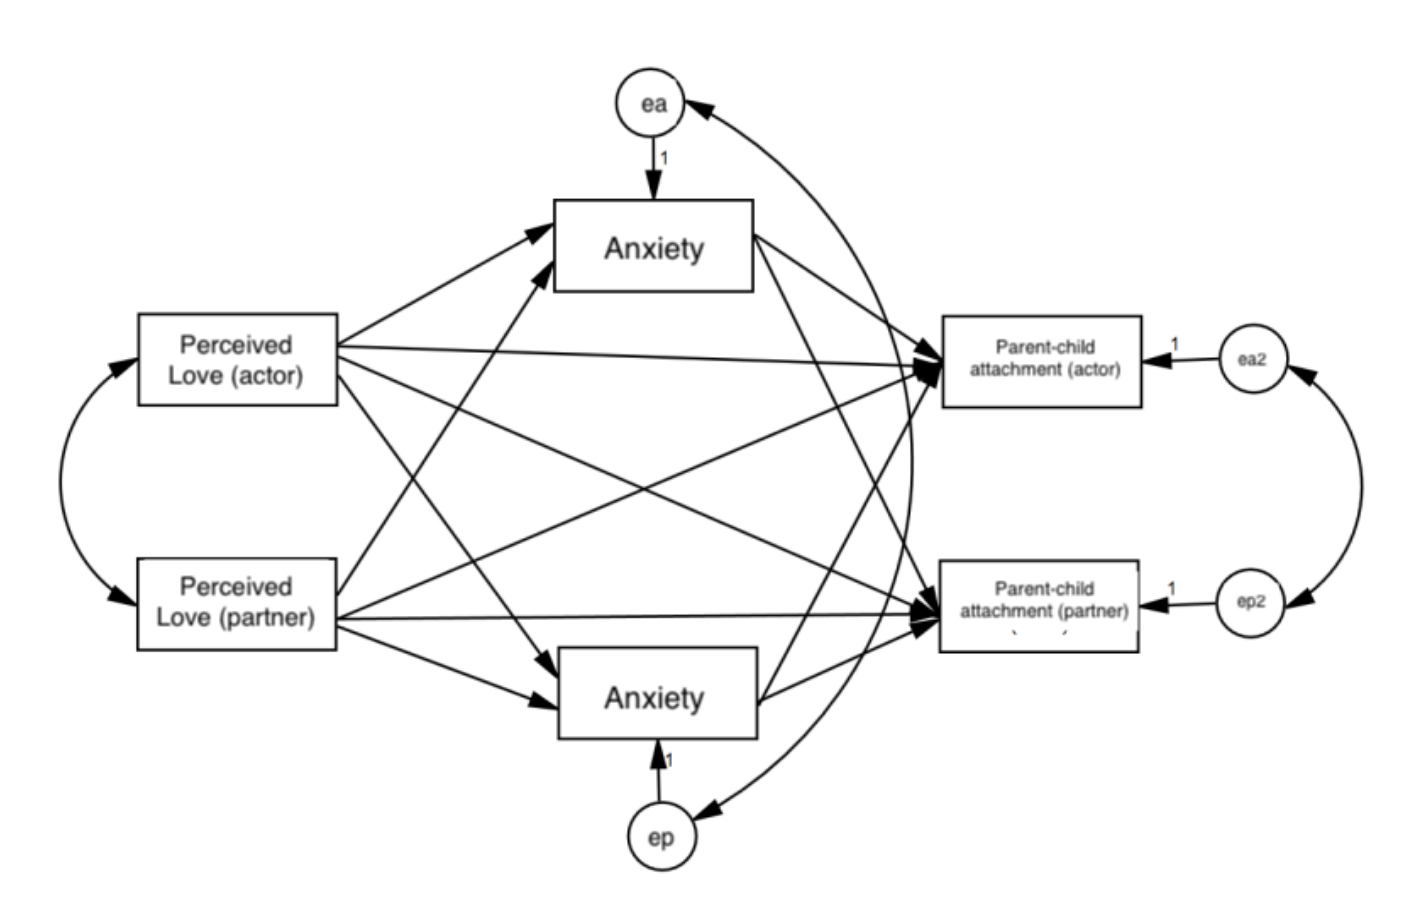
\includegraphics[width=500px]{figure1} 

}

\caption{Love and attachment mediated by anxiety}\label{fig:unnamed-chunk-1}
\end{figure}

\begin{figure}

{\centering 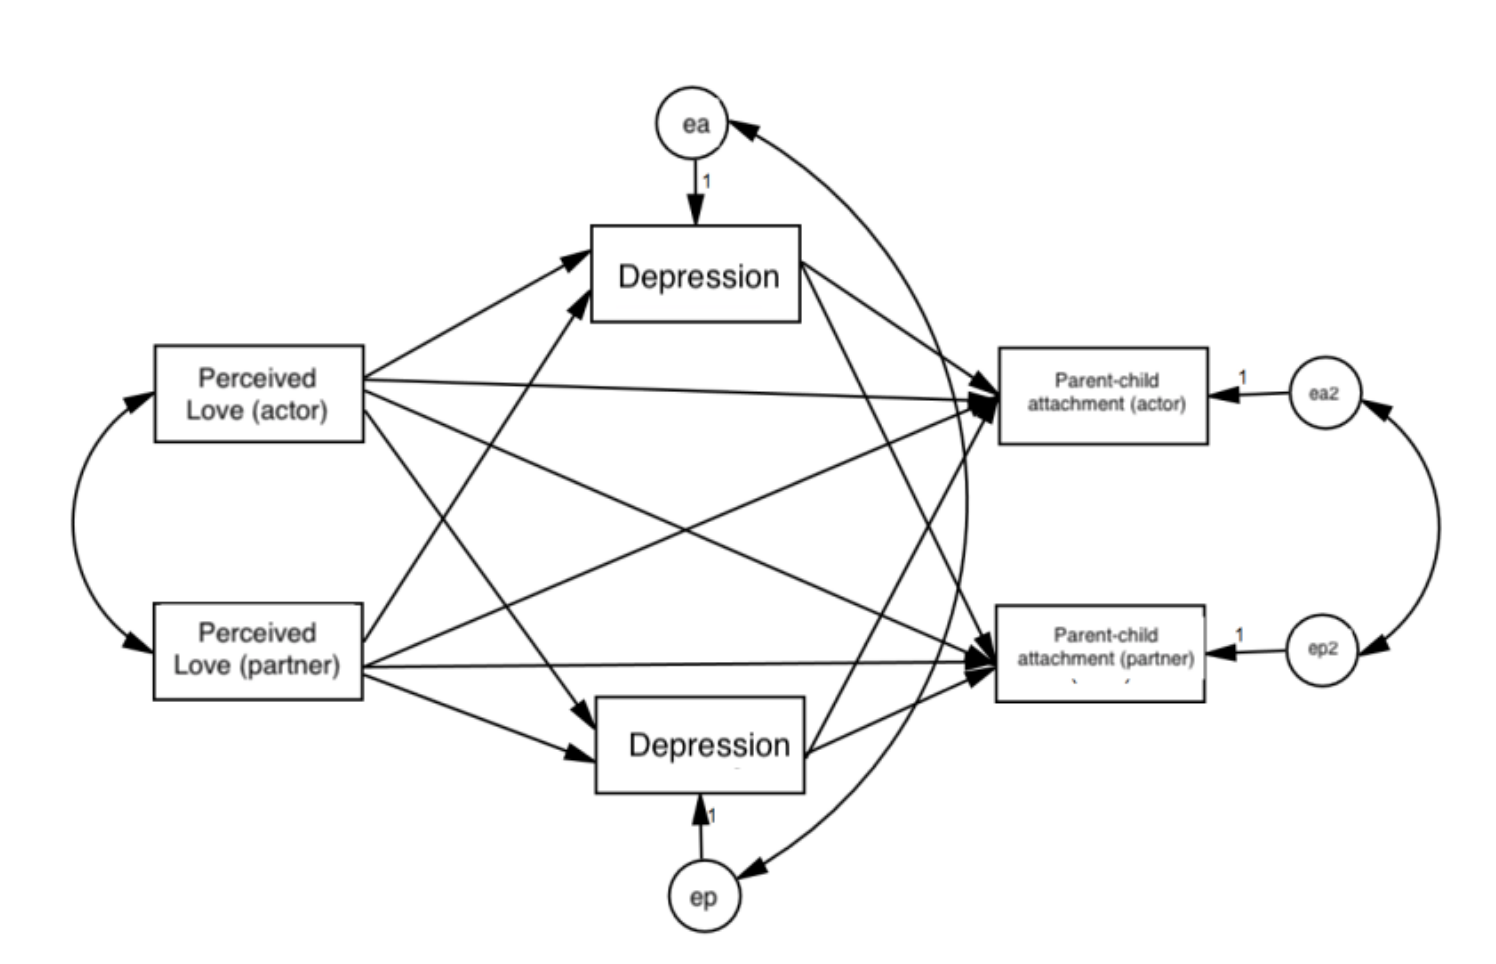
\includegraphics[width=500px]{figure2} 

}

\caption{Love and attachment mediated by depression}\label{fig:unnamed-chunk-2}
\end{figure}

\begin{table}[tbp]

\begin{center}
\begin{threeparttable}

\caption{\label{tab:unnamed-chunk-16}Predicting attachment with time and love}

\begin{tabular}{llllll}
\toprule
 & \multicolumn{1}{c}{Value} & \multicolumn{1}{c}{Std.Error} & \multicolumn{1}{c}{DF} & \multicolumn{1}{c}{t-value} & \multicolumn{1}{c}{p-value}\\
\midrule
(Intercept) & 3.45 & 0.20 & 572.00 & 17.45 & 0.00\\
time & 0.00 & 0.01 & 572.00 & -0.06 & 0.95\\
love\_A & 0.11 & 0.02 & 572.00 & 5.98 & 0.00\\
love\_P & -0.02 & 0.02 & 572.00 & -0.83 & 0.41\\
\bottomrule
\end{tabular}

\end{threeparttable}
\end{center}

\end{table}

\begin{table}[tbp]

\begin{center}
\begin{threeparttable}

\caption{\label{tab:unnamed-chunk-17}Predicting attachment with time and love and group*love interaction}

\begin{tabular}{llllll}
\toprule
 & \multicolumn{1}{c}{Value} & \multicolumn{1}{c}{Std.Error} & \multicolumn{1}{c}{DF} & \multicolumn{1}{c}{t-value} & \multicolumn{1}{c}{p-value}\\
\midrule
(Intercept) & 3.71 & 0.29 & 568.00 & 12.80 & 0.00\\
time & 0.00 & 0.01 & 568.00 & -0.08 & 0.93\\
love\_A & 0.06 & 0.03 & 568.00 & 1.97 & 0.05\\
groupgay & -0.75 & 0.50 & 138.00 & -1.48 & 0.14\\
grouples & -0.27 & 0.43 & 138.00 & -0.64 & 0.52\\
love\_P & 0.00 & 0.03 & 568.00 & 0.12 & 0.90\\
love\_A:groupgay & 0.12 & 0.05 & 568.00 & 2.58 & 0.01\\
love\_A:grouples & 0.07 & 0.05 & 568.00 & 1.47 & 0.14\\
groupgay:love\_P & -0.02 & 0.05 & 568.00 & -0.51 & 0.61\\
grouples:love\_P & -0.02 & 0.05 & 568.00 & -0.47 & 0.64\\
\bottomrule
\end{tabular}

\end{threeparttable}
\end{center}

\end{table}

\hypertarget{results}{%
\section{Results}\label{results}}

\hypertarget{analysis-strategy}{%
\subsection{Analysis Strategy}\label{analysis-strategy}}

We hypothesized that the individuals' perception of love and their partner's perception of love in their relationship would affect the parent-child relationship positively and associations would become stronger over time (hypothesis 1). We also hypothesized that the correlation between love and parent-child attachment would be different across family types (hypothesis 2). Furthermore, we hypothesized that depressive and anxiety symptoms play mediating roles in the association between love and attachment (hypotheses 3 and 4). We used multilevel modeling and the Actor-Partner Interdependence Model (APIM; Kenny, Kashy, and Cook (2006)) to test these hypotheses. The APIM simultaneously estimates the effect of one's perception of love in the relationship and the effect of the same variable but from the partner on parent-child attachment. Since our data was divided into three waves, the growth curve model was used. Given the characteristics of APIM and longitudinal data, we need to check for the intercept covariance, slope covariance, and slope-intercept covariance.
In our first hypothesis we used the following explanatory variables: 1) the actor's perception of love in the relationship, 2) partner's perception of love in the relationship, 4) time. The response variable was actor's attachment. In our second hypothesis we added an interaction between love and actor-partner relationship type (lesbian, gay, or hetersexual).
In our third and fourth hypothesis we tested whether anxiety and depression of the actor could be potential mediators between the correlation of love of the actor and the actor's perceived attachment. Figures 1 and 2 provide a visual examples of what mediation looks like within a APIM. We used the Monte Carlo method (Tofighi \& MacKinnon, 2011) for assessing mediation which created confidence intervals for indirect effects.

\hypertarget{main-results}{%
\subsection{Main Results}\label{main-results}}

\hypertarget{hypothesis-1}{%
\subsubsection{Hypothesis 1:}\label{hypothesis-1}}

In our first model, there was a statistically significant effect of the individuals' perception of love on the perceived parent-child attachment for that individual, such that the higher the perception of love the more the person perceived that they were attached to their children, b = 0.11, SE = 0.019, p = 0.000. Nevertheless, a person's partner's perception of love in their relationship did not show statistically significant effects on neither themselves's nor their partner's perceived parent-child attachment. We also found that time was not a statistically significant moderator for the correlation between love and attachment, such as the correlation between love and attachment for a person at time point one does not predict the correlation between love and attachment for a person at the following time point. In the model the intercept variance was 0.05, intercept covariance was 0.02, and correlation between intercepts was 0.33. In regards to slope, the slope variance was 0.00, the slope covariance was 0.00, correlation between the slopes was 0.95, slope-intercept covariance (within a person) was 0.00, slope-intercept correlation (within a person) was 0.72, slope-intercept covariance (between persons) was 0.01, and slope-intercept correlation (between a person) was 0.89.Further details on the outcomes for the hypothesis test are provided in Table 1.

\hypertarget{hypothesis-2}{%
\subsubsection{Hypothesis 2:}\label{hypothesis-2}}

For our second hypothesis, we predicted that the correlations of perception of love and parent-child attachment would be different across family types. Contradict to our prediction, we did not find the interaction of different family types on the correlation between love and parent-child attachment with respect to time point statistically significant. In the model, the intercept variance was 0.05, intercept covariance was 0.02, and correlation between intercepts was 0.29. In regards to slope, the slope variance was 0.00, the slope covariance was 0.00, correlation between the slopes was 0.97, slope-intercept covariance (within a person) was 0.00, slope-intercept correlation (within a person) was 0.72, slope-intercept covariance (between persons) was 0.01, and slope-intercept correlation (between a person) was 0.87. Further details on the outcomes for the hypothesis test one are provided in Table 2.

\hypertarget{hypothesis-3}{%
\subsubsection{Hypothesis 3:}\label{hypothesis-3}}

In order to determine if anxiety mediates the relationship between perceived love in the parental relationship and parent-child relationship, a series of regression analyses were conducted. First, the love reported in the parental relationship (b = 0.11, SE = 0.041, p = 0.0000) significantly predicted parent-child attachment. Next, we found that the trait of anxiety was significantly predicted by an individual's perception of love in the relationship (b = -0.11, SE = 0.021, p = 0.0000). Finally, we found that an individual's perception of love (b = 0.067, SE = 0.022, p = 0.0032) and the trait of anxiety (b = -0.33, SE = 0.046, p = 0.0000) together significantly predicted parent-child attachment. The results revealed that anxiety negative mediated the relationship between the perceived love in one's relationship and the perceived attachment to one's child. Finally, we used the Monte Carlo method (Tofighi \& MacKinnon, 2011) and found that the indirect effect of the mediation is statistically significant (CI ranges from 0.0199 to 0.0524).

\hypertarget{hypothesis-4}{%
\subsubsection{Hypothesis 4:}\label{hypothesis-4}}

In our fourth model, we found that there was a statistically significant mediation effect of depression on the correlation between love and attachment. In our previous model, we learned that there was a significant correlation between the actor's love and the actor's attachment. Then we tested and found that there was a statically significant actor effect of love on depression, such that the actor's depression level decreased with the increase of their own perceived love, b = -0.098, SE = 0.019, p = 0.000. We further tested the direct effect of actor's love and their depression on attachment in a full model and found that both the actor effect of love(b = 0.077, SE = 0.023, p = 0.0008) and depression(b = -0.27, SE = 0.046, p = 0.0000) were statistically correlated with attachment. This mediation was such that a person who was high in perceived love had a lower level of depression, while a higher level of depression also negatively influence their perceived parent-child attachment. Finally, we used the Monte Carlo method (Tofighi \& MacKinnon, 2011) and found that the indirect effect of the mediation is statistically significant (CI ranges from 0.0194 to 0.0532).
In the full model, we also found time as a statistically significant predictor for the correlation between depression and love to attachment (b = -0.065, SE = 0.032, p = 0.043); however, we deduced the significance to be inconclusive since we did not find significant correlation with either attachment or love.

\newpage

\hypertarget{references}{%
\section{References}\label{references}}

\begingroup
\setlength{\parindent}{-0.5in}
\setlength{\leftskip}{0.5in}

\hypertarget{refs}{}
\leavevmode\hypertarget{ref-apim}{}%
Kenny, D. A., Kashy, D. A., \& Cook, W. L. (2006). \emph{Dyadic data analysis}. Guilford press.

\leavevmode\hypertarget{ref-monte}{}%
Tofighi, D., \& MacKinnon, D. P. (2011). RMediation: An r package for mediation analysis confidence intervals. \emph{Behavior Research Methods}, \emph{43}(3), 692--700.

\endgroup


\end{document}
